\begin{frame}{Aufgabe 4: Änderung des Empfangsfilters}
  \twocolumns{
    \[B = 2.76 \, \si{\kilo\hertz}\]
    \[U_\mathrm{A}=0.8651 \, \si{\volt}\]
    \[P_\mathrm{R}=0.09861 \, \si{\volt}^2\]
    \[\rho = \frac{U_\mathrm{A}^2}{P_\mathrm{R}} = 7.59\]
    \[\textrm{BER} = 2.9 \cdot 10^{-3}\]
    \[\textrm{BER}_g = 1.7036 \cdot 10^{-3}\]
    }{
  \begin{center}
  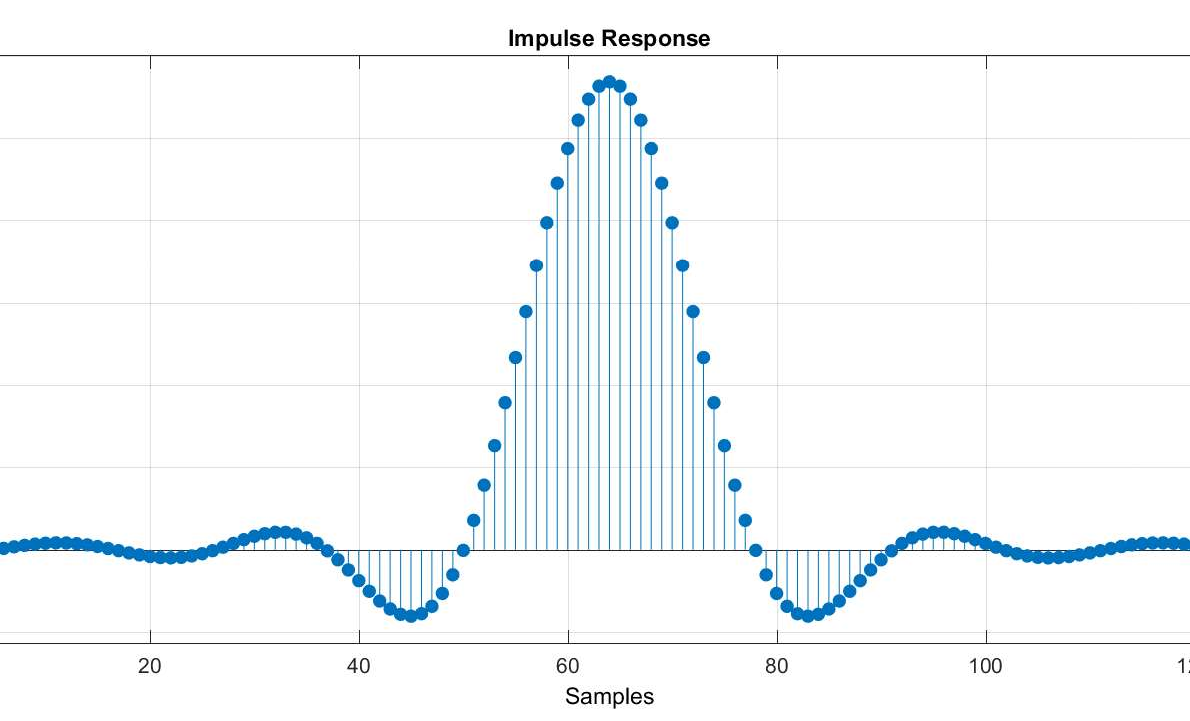
\includegraphics[width=\textwidth]{screenshots/Aufgabe4/sendefilter_impulsantwort}
  \end{center}
  }{0.5\textwidth}
\end{frame}

\begin{frame}{Aufgabe 4: Änderung des Empfangsfilters}
  \[g_{\mathrm{ef}}(t) \neq g_\mathrm{s}(-t)\]
\end{frame}